\documentclass[11pt,a4paper]{article}

\usepackage[utf8]{inputenc}
\usepackage[T1]{fontenc}
\usepackage[spanish]{babel}

\usepackage{tgpagella}
\usepackage{geometry}
\usepackage{booktabs}
\usepackage{xcolor}
\usepackage{graphicx}
\usepackage{titlesec}
\usepackage{fancyhdr}
\usepackage[parfill]{parskip}
\usepackage[expansion=false]{microtype}
\usepackage{hyperref}
\usepackage{setspace}
\usepackage{needspace}
\usepackage{etoolbox}
\usepackage{ragged2e}

\widowpenalty=10000
\clubpenalty=10000
\displaywidowpenalty=10000

\hyphenpenalty=8000
\exhyphenpenalty=8000

\geometry{top=3.0cm,bottom=3.0cm,left=3.5cm,right=3.5cm}

\setlength{\parskip}{0.65em}
\setlength{\parindent}{0em}

\definecolor{azulai}{RGB}{30,80,140}
\definecolor{doradoai}{RGB}{140,90,0}
\definecolor{grisai}{RGB}{70,70,70}

\AtBeginDocument{\justifying}

\titleformat{\section}
{\Large\bfseries\color{azulai}\\justifying}
{}
{0em}
{}
[{\color{azulai}\titlerule[0.5pt]}]

\titlespacing*{\section}
{0pt}{1.3em}{0.5em}

\titleformat{\subsection}
{\large\bfseries\color{doradoai}\\justifying}
{}
{0em}
{}

\titlespacing*{\subsection}
{0pt}{1.0em}{0.35em}

\titleformat{\subsubsection}
{\normalsize\bfseries\color{grisai}\\justifying}
{}
{0em}
{}

\titlespacing*{\subsubsection}
{0pt}{0.8em}{0.25em}

\preto\section{\Needspace{8\baselineskip}}
\preto\subsection{\Needspace{6\baselineskip}}
\preto\subsubsection{\Needspace{4\baselineskip}}

\pagestyle{fancy}
\fancyhf{}

\rhead{\textcolor{grisai}{\small jk — Arquitectura Interna}}
\lhead{\textcolor{grisai}{\small Mercurio · Venus · Marte}}
\cfoot{\textcolor{grisai}{\small\thepage}}

\renewcommand{\headrulewidth}{0.3pt}

\hypersetup{
colorlinks=true,
linkcolor=azulai,
urlcolor=azulai
}

\setstretch{1.32}

\tolerance=1500
\emergencystretch=4em

\begin{document}

% ── Portada ──────────────────────────────────────────────────────────────────

\begin{titlepage}
  \centering

  \vspace*{2cm}

  {\Huge\bfseries\color{azulai} Mercurio · Venus · Marte}\\[0.6cm]

  {\large\color{grisai} Arquitectura Interna}\\[0.4cm]

  {\small\itshape\color{grisai}
  Procesamiento, vínculo y acción en el funcionamiento cotidiano
  }\\[2.2cm]

  {\huge\color{doradoai} jk}\\[1.6cm]

  {\Large 15/04/1599 \quad 04:52}\\[0.35cm]

  {\Large dsaf}\\[0.35cm]

  {\normalsize
  Lat: 42.9427° \quad
  Lon: -2.6441° \quad
  UTC-00:15
  }\\[0.35cm]

  {\normalsize
  Ascendente: Aries 12°35'
  \quad
  MC: Capricornio 6°21'
  }\\[2.2cm]

  \renewcommand{\arraystretch}{1.35}

  \begin{tabular}{ll}
    \textbf{Mercurio:} & Aries — Casa 12 6°39' \\
    \textbf{Venus:}    & Tauro — Casa 1 5°26' \\
    \textbf{Marte:}    & Piscis — Casa 12 25°13' \\
  \end{tabular}

  \vfill

  {\small\color{grisai}
  Generado el 20/05/2026
  }

\end{titlepage}

\\justifying

\tableofcontents

\clearpage

% ── Datos de referencia ───────────────────────────────────────────────────────
\section{Datos de referencia}

\begin{center}
\renewcommand{\arraystretch}{1.25}
\begin{tabular}{llll}
  \toprule
  \textbf{Planeta} & \textbf{Signo} & \textbf{Casa} & \textbf{Posición} \\
  \midrule
  Mercurio  & Aries  & 12  & 6°39' \\
  Venus    & Tauro & 1 & 5°26' \\
  Marte    & Piscis & 12 & 25°13' \\
  Ascendente          & Aries           & ---                    & 12°35' \\
  Medio Cielo         & Capricornio            & ---                    & 6°21' \\
  \bottomrule
\end{tabular}
\end{center}
\\justifying

\vspace{0.5cm}

\textbf{Aspectos entre planetas personales:}

\vspace{0.3cm}\textit{No hay aspectos entre los planetas personales en los orbes definidos.}

\\justifying

\vspace{0.7cm}

\begin{center}
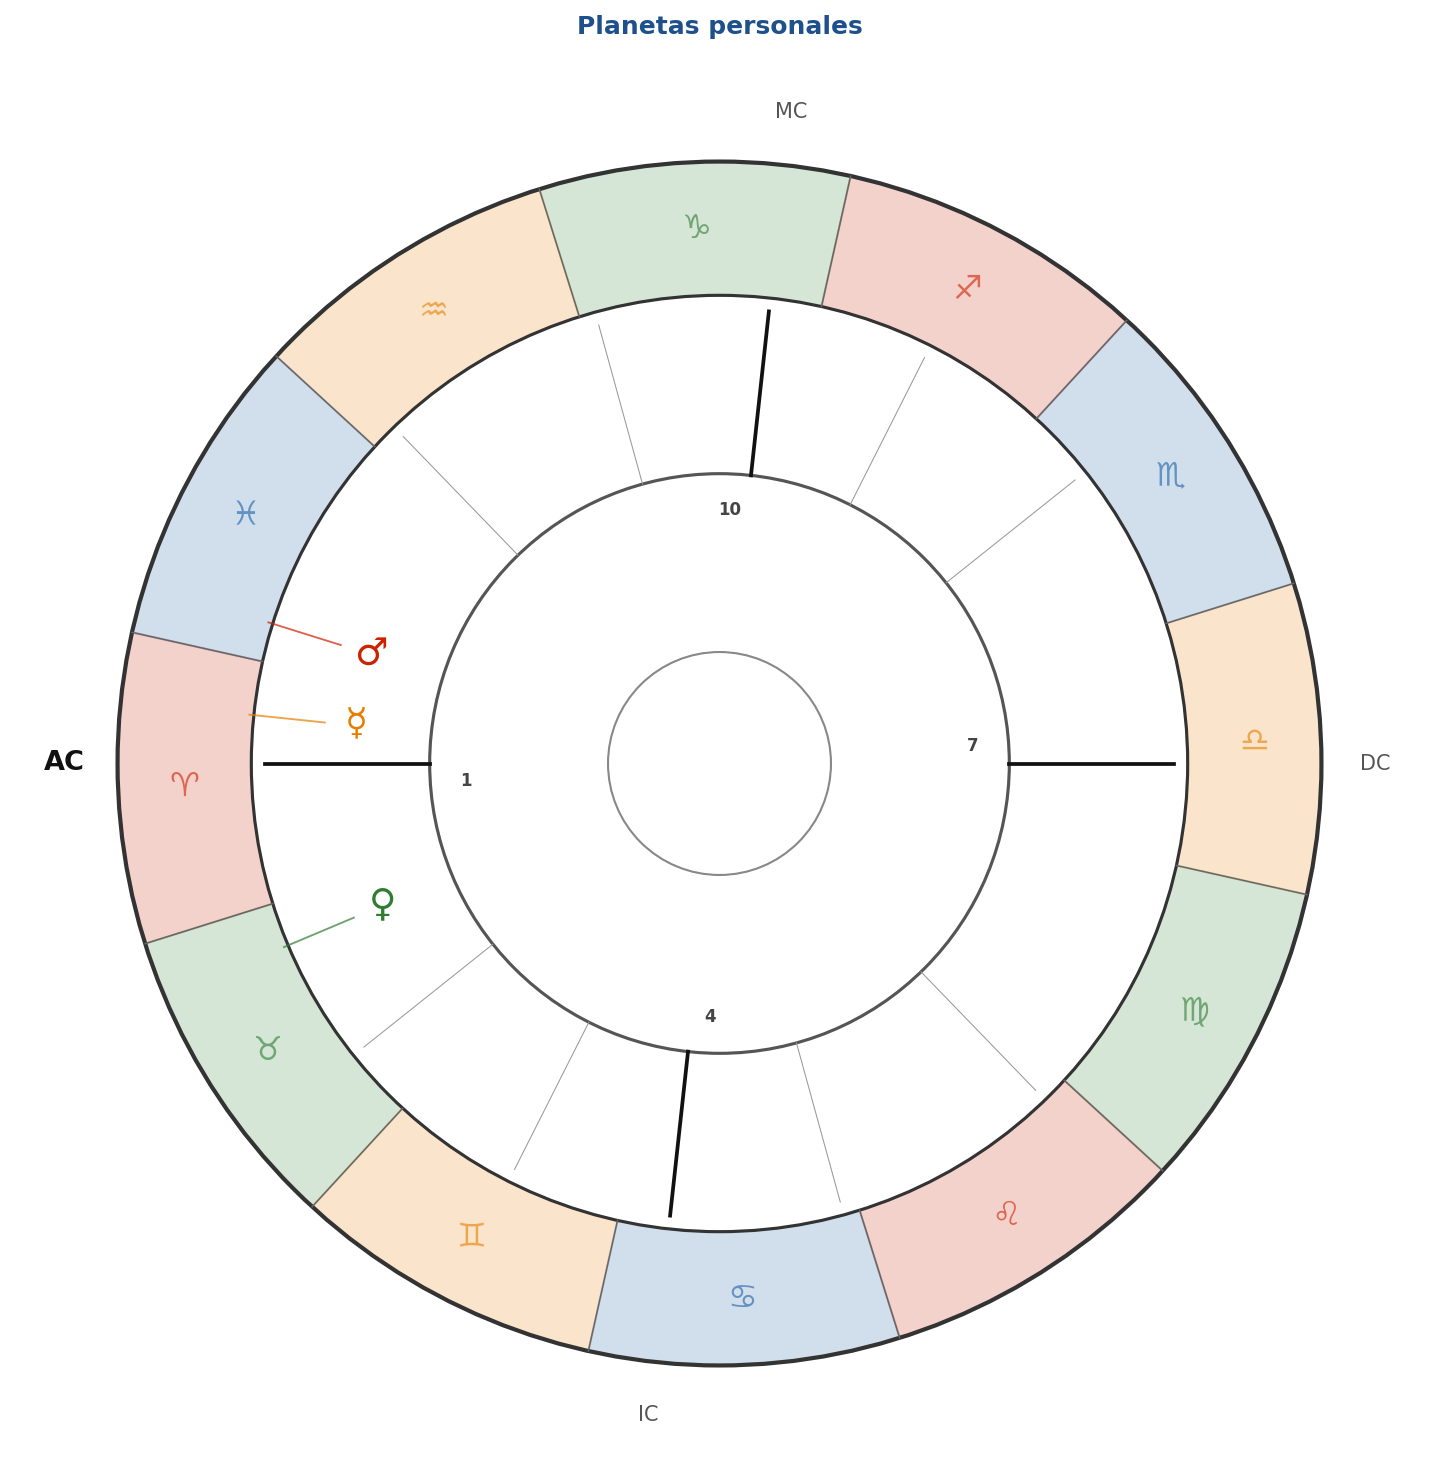
\includegraphics[width=0.72\textwidth]{jk_Planetas_Personales_rueda.png}
\end{center}

\vspace{0.3cm}
\Needspace{5\baselineskip}

% ── Interpretación ────────────────────────────────────────────────────────────
\section{Interpretación — Arquitectura Interna}

\begin{center}
{\small\itshape\color{grisai}
No se trata de describir la personalidad.\\
Se trata de observar cómo procesas, cómo te vinculas\\
y cómo se mueve tu energía en la vida cotidiana.
}
\end{center}

\\justifying

\vspace{0.8cm}

% ── 1. Funcionamiento general ─────────────────────────────────────────────────
\subsection{1. Funcionamiento general}

\\justifying
Mercurio está en Aries, Casa 12: muestra cómo piensas, cómo ordenas lo que percibes y cómo traduces lo que ocurre en palabras o ideas.
Venus está en Tauro, Casa 1: muestra cómo te vinculas, qué necesitas para sentir conexión y cómo buscas equilibrio afectivo.
Marte está en Piscis, Casa 12: muestra cómo se activa tu acción, cómo descargas energía y cómo respondes ante el impulso.

Hay coherencia elemental entre: tu forma de vincularte (Venus) y tu forma de actuar (Marte) se apoyan por elementos compatibles: Tierra/Agua. Esto facilita que esas áreas colaboren entre sí. Aun así, lo que fluye con facilidad también puede volverse automático si no lo observas con consciencia.

Hay tensión elemental entre: tu forma de pensar (Mercurio, Fuego) y tu forma de vincularte (Venus, Tierra); tu forma de pensar (Mercurio, Fuego) y tu forma de actuar (Marte, Agua). Esto no es un problema en sí mismo, pero sí pide más atención. Cuando esas áreas necesitan cooperar, conviene hacer una integración consciente para que una no bloquee, desborde o desconecte a la otra.

No aparecen aspectos clásicos entre los planetas personales dentro de los orbes definidos. Aun así, puede existir una concentración funcional si los planetas están próximos por signo, por casa o por continuidad de experiencia.

\vspace{0.8cm}

% ── 2. Mercurio ───────────────────────────────────────────────────────────────
\subsection{2. Mercurio — Pensamiento y procesamiento}

\subsubsection*{Mercurio en Aries — Casa 12}

\\justifying
Tu mente funciona rápido y tiende a llegar a una conclusión antes de haber revisado todo el proceso. Sueles responder primero y comprobar después. Esto aporta rapidez real, capacidad de reacción y facilidad para decidir en movimiento.

La saturación aparece cuando hay demasiada información sin una prioridad clara. Si todo parece urgente al mismo tiempo, la velocidad se convierte en impaciencia y puedes actuar antes de haber terminado de entender. El bloqueo suele aparecer cuando hay que esperar, repetir algo varias veces o explicar en detalle algo que internamente ya sentías resuelto.

Sueles pensar mejor cuando puedes avanzar por pasos cortos, tomar decisiones concretas y descargar mentalmente la información mediante acción.

Necesitas silencio, soledad y pausas profundas para ordenar la mente. Procesas lentamente hacia adentro y muchas veces necesitas tiempo antes de comprender del todo lo que piensas o sientes. Las ideas suelen madurar en espacios internos más que en estímulos constantes.

La saturación aparece cuando hay demasiado ruido mental, exposición o actividad continua sin descanso psicológico. Entonces la claridad disminuye y puedes sentir la mente más difusa o dispersa. Sueles pensar mejor cuando existen momentos de retiro, descanso mental y tiempo sin exigencia cognitiva.

\vspace{0.8cm}

% ── 3. Venus ──────────────────────────────────────────────────────────────────
\subsection{3. Venus — Vínculo y regulación relacional}

\subsubsection*{Venus en Tauro — Casa 1}

\\justifying
Necesitas estabilidad, continuidad y presencia real para sentir seguridad en el vínculo. Las relaciones suelen construirse lentamente y fortalecerse a través de la constancia, el contacto y la sensación de que la otra persona permanece.

La saturación aparece cuando hay cambios bruscos, señales contradictorias o inestabilidad emocional sostenida. Entonces puedes empezar a cerrarte para protegerte. Cuando el vínculo deja de sostenerse, la desconexión suele ser gradual más que explosiva: la apertura disminuye poco a poco hasta que volver a confiar requiere demasiado esfuerzo.

Sueles regularte mejor mediante estabilidad, tiempo compartido y relaciones donde las acciones coinciden con las palabras.

Necesitas presencia directa y contacto cercano para sentir viva la conexión. Sueles relacionarte de forma visible, espontánea y bastante inmediata. Poder mostrarte tal como eres y sentirte realmente viste forma parte importante de tu regulación afectiva.

La saturación aparece cuando sientes que tienes que esconder demasiado quién eres o sostener una imagen artificial durante mucho tiempo. Sueles regularte mejor en vínculos donde existe naturalidad, presencia real y espacio para expresarte sin excesiva contención.

\vspace{0.8cm}

% ── 4. Marte ──────────────────────────────────────────────────────────────────
\subsection{4. Marte — Acción y descarga}

\subsubsection*{Marte en Piscis — Casa 12}

\\justifying
Tu energía se activa de forma sensible y cambiante. Muchas veces no actúas desde impulso directo, sino desde estados internos, intuiciones o conexión emocional con lo que ocurre alrededor. La acción descarga mejor mediante creatividad, ayuda, arte o actividades con dimensión emocional o espiritual.

La saturación aparece cuando la energía no encuentra dirección clara o absorbes demasiado del entorno. Entonces aparece pasividad, dispersión o dificultad para actuar desde una decisión propia. La acción puede quedar reemplazada por adaptación constante a lo que otras personas necesitan.

Sueles regularte mejor mediante descanso, espacios creativos, movimiento suave y actividades que permitan conectar con sentido interno.

Tu energía tiende a funcionar hacia adentro y no siempre encuentra salida visible inmediata. Puedes acumular activación silenciosamente si no existen espacios seguros de descarga.

La saturación aparece cuando toda la energía queda retenida internamente o te adaptas constantemente a lo que otras personas necesitan sin registrar tu propio impulso. Entonces aparece agotamiento, confusión o sensación de pérdida de dirección. Sueles regularte mejor mediante descanso profundo, creatividad, práctica interior y actividades donde puedas actuar sin exceso de exposición externa.

\vspace{0.8cm}

% ── 5. Integración ────────────────────────────────────────────────────────────
\subsection{5. Integración — Coherencias, fricciones y bucles}

\\justifying
Mercurio (Aries, Fuego) y Venus (Tauro, Tierra) operan en elementos que crean tensión. Lo que necesitas para procesar y lo que necesitas para vincularte no siempre siguen la misma lógica.

Mercurio (Aries, Fuego) y Marte (Piscis, Agua) operan en elementos que crean tensión. Tu modo de procesar y tu modo de actuar no se alimentan de forma directa. Puede haber mucho pensamiento sin movimiento, o acción antes de que exista claridad suficiente.

Cuando hay demasiada presión, puede aparecer una cadena reconocible: Mercurio en Aries acelera hacia conclusiones antes de que el análisis esté completo. Desde ahí, Venus en Tauro se cierra lentamente y deja de estar disponible. Y Marte en Piscis se disipa o actúa en dirección del entorno antes que desde el propio impulso. El ciclo se cierra cuando la energía acumulada vuelve a saturar el punto inicial.

\vspace{0.8cm}

% ── 6. Orientación práctica ───────────────────────────────────────────────────
\subsection{6. Orientación práctica}

\subsubsection*{Desde dónde empezar}

\\justifying
Desde tu forma de pensar (Mercurio) en Aries, Casa 12. De las tres áreas, esta suele requerir menos energía para activarse. La entrada es activar el movimiento antes de intentar resolverlo todo mentalmente. Empezar por aquí puede abrir movimiento en el resto.

\subsubsection*{Qué sostener}

\\justifying
Conviene sostener especialmente tu forma de actuar (Marte) en Piscis: tiempo de integración, silencio emocional y límites sensibles. Bajo presión, esta área puede desorganizarse antes que las demás. Cuando se estabiliza, el resto de tu funcionamiento tiene más capacidad para reorganizarse.

\subsubsection*{Qué evitar}

\\justifying
Evitar asumir que la ausencia de fricción visible significa que todo está bien. A veces los bucles no hacen ruido porque te has acostumbrado a funcionar así.

\vspace{0.6cm}

\\justifying
Si no se sostiene: pensamiento, vínculo y acción empiezan a funcionar por separado. Lo que piensas no alimenta la acción, la acción no informa al vínculo y el vínculo no regula la energía disponible. El esfuerzo aumenta, la claridad disminuye y la saturación llega antes.

\vspace{1.2cm}

\begin{center}
{\small\itshape\color{grisai}
La astrología se utiliza aquí como lenguaje simbólico de observación,\\
no como una definición cerrada de quién eres.\\[0.2cm]
Este documento propone una lectura funcional y orientativa, no un diagnóstico.
}
\end{center}

\end{document}
